\documentclass[english,svgnames,notes=hide,12pt]{beamer}
\usepackage{macros-ohp}

\def\seminarname{Machine Learning Seminar}
\def\presentationtitle{Introducci\'on a Machine Learning}

\title{\large\seminarname:\\\large\presentationtitle}
\author{Berthin Torres \& Rodolfo Quispe\\
    \small University of Campinas
}

% Fill the date or leave it blank to not display it
\date{January 28th, 2019}

\begin{document}
\thispagestyle{empty}
\begin{frame}
    \titlepage
\end{frame}

\begin{frame}
    \frametitle{Outline}
    \tableofcontents
\end{frame}

\AtBeginSection[]
{
    \begin{frame}<beamer>
    \frametitle{Outline}
    \tableofcontents[currentsection]
    \end{frame}
}

\section{Machine Learning Foundations}
\begin{frame}
    \begin{figure}
        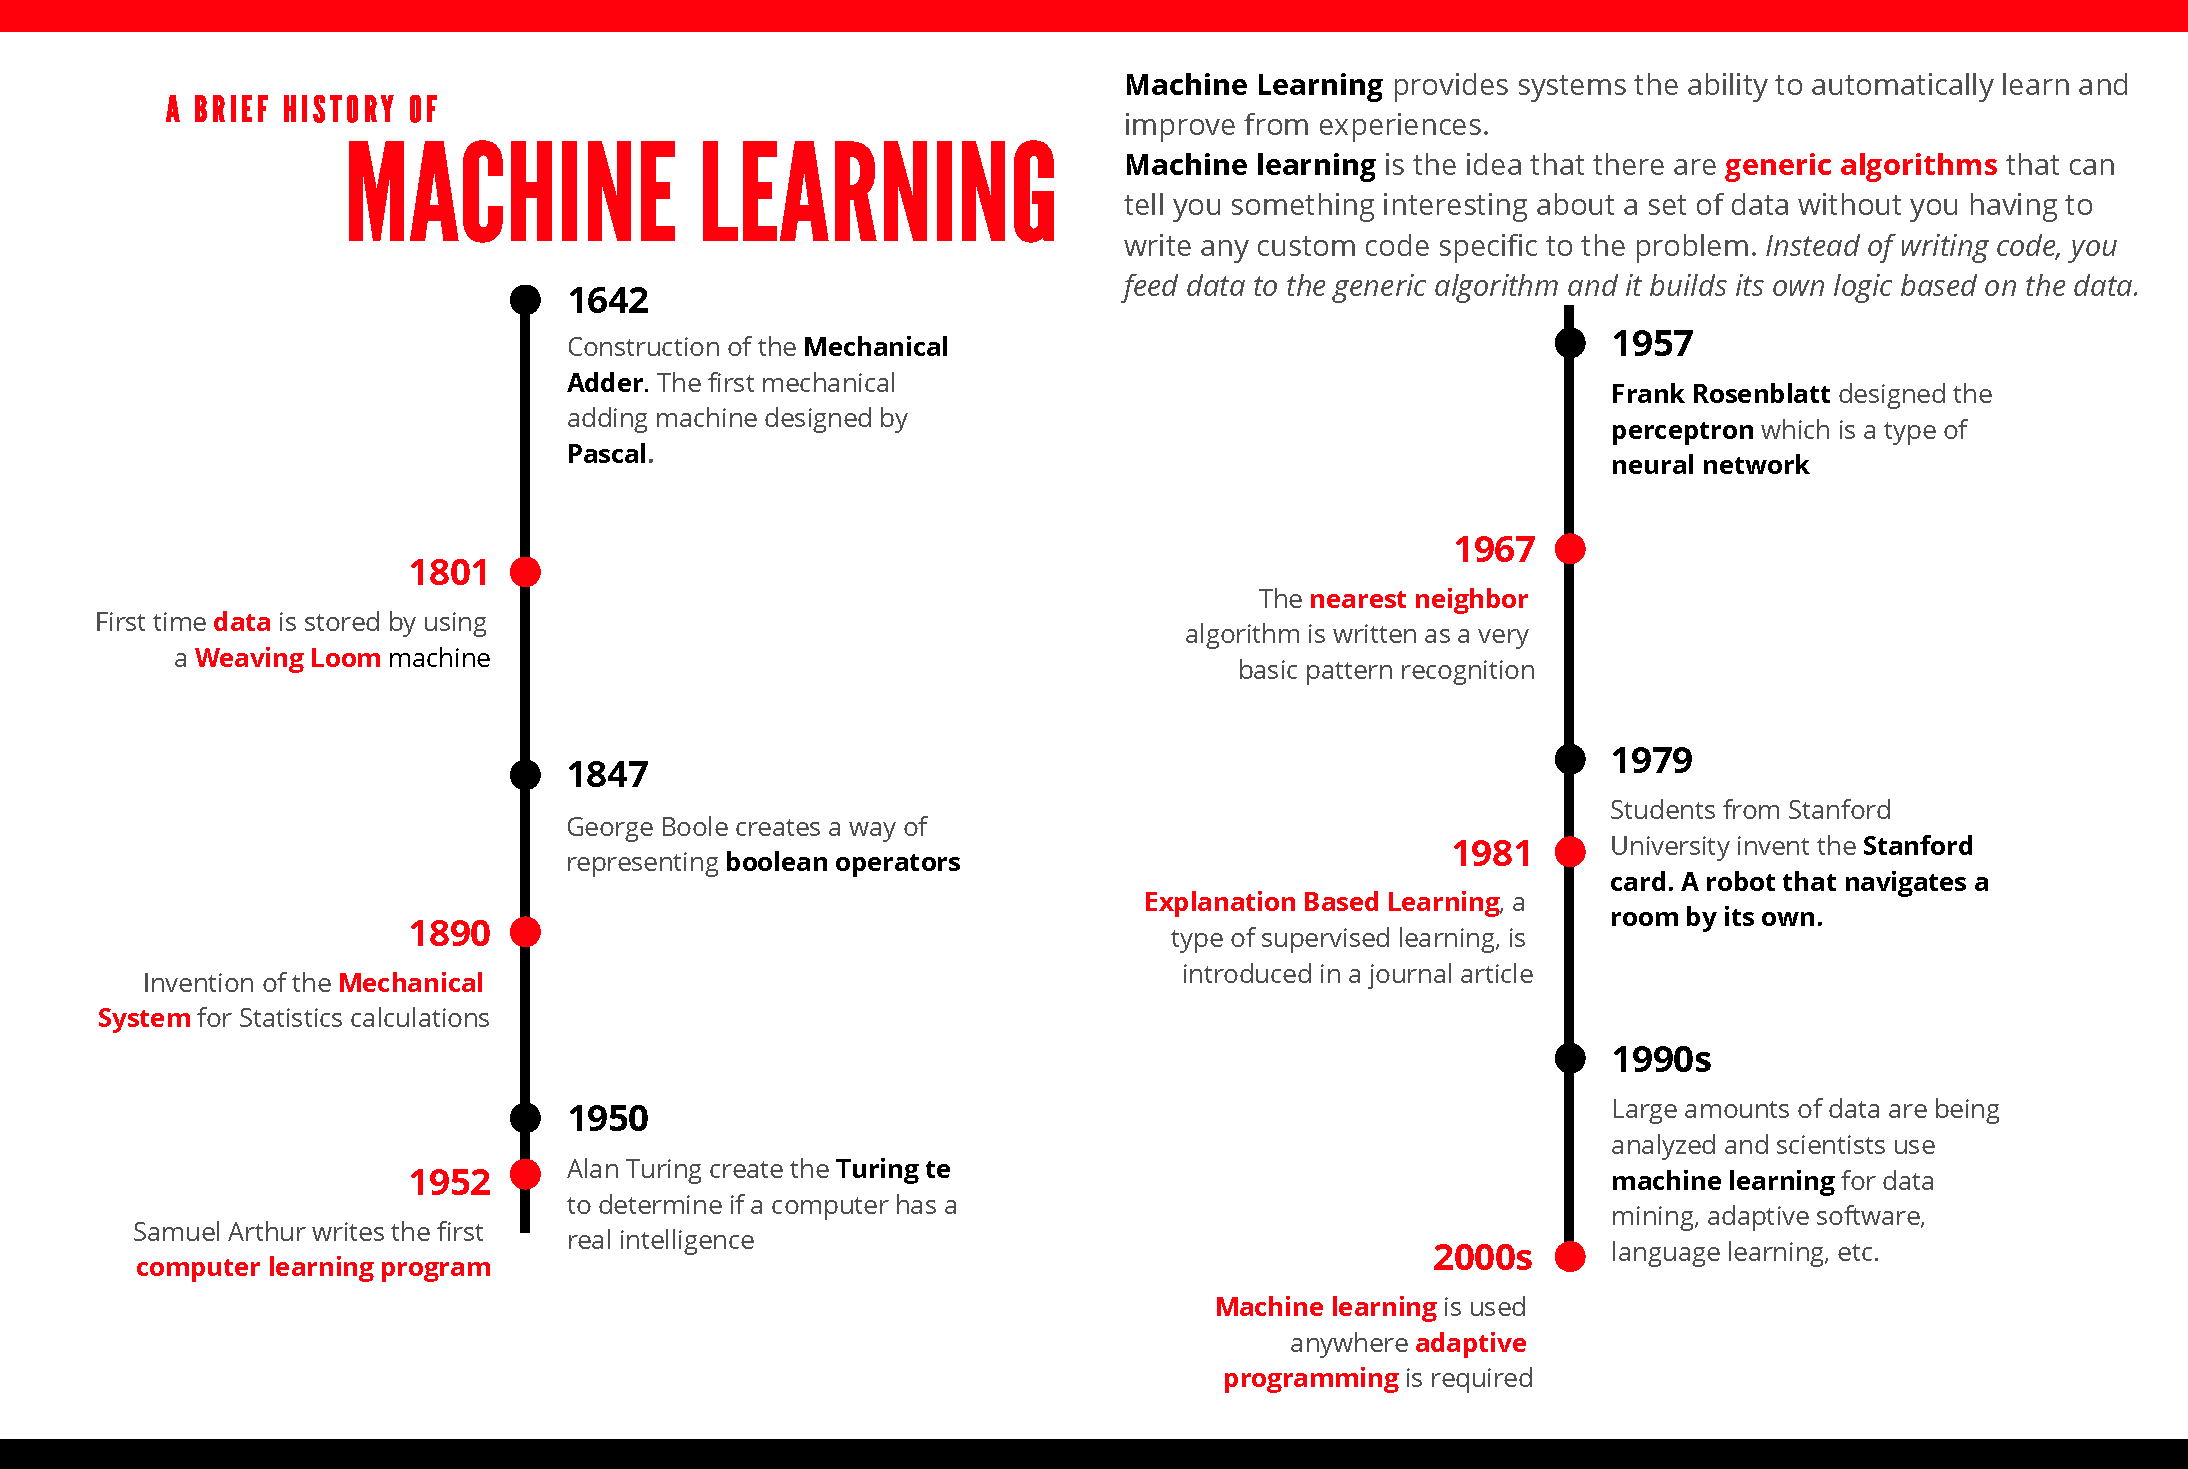
\includegraphics[width=0.8\textwidth]{imgs/machine-learning-timeline.pdf}
    \end{figure}
    \centering\tiny{Source: \url{https://medium.com/bloombench/history-of-machine-learning-7c9dc67857a5}}
\end{frame}

\begin{frame}
    \textbf{Machine Learning} es un enfoque para crear algoritmos genericos que sean capaces de aprender patrones o relaciones de un conjunto de informaci\'on.
    \vspace{-.5cm}
    \begin{figure}
        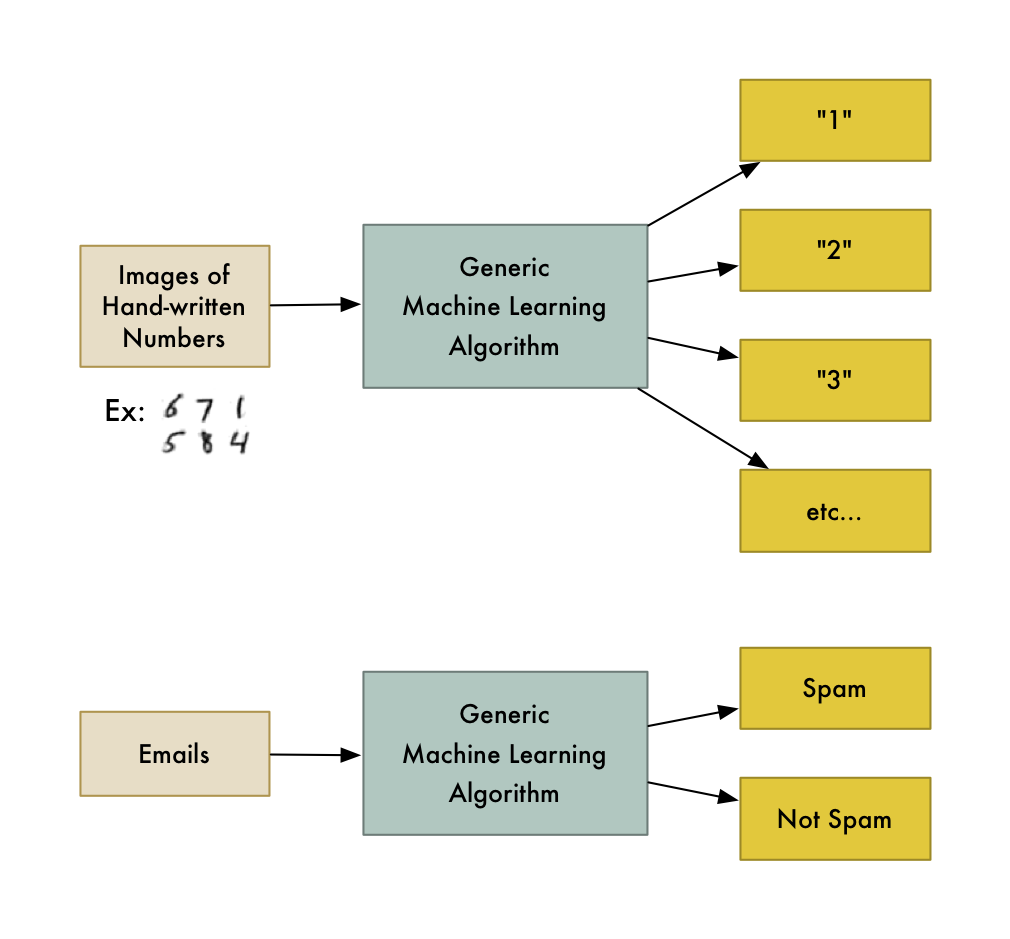
\includegraphics[width=0.5\textwidth]{imgs/sample-ml.png}
    \end{figure}
    \vspace{-.5cm}
    \centering\tiny{Source: \url{https://medium.com/@ageitgey/machine-learning-is-fun-80ea3ec3c471}}
\end{frame}

%\setbeamercovered{transparent}
\begin{frame}
\begin{table}[]
    \caption{Informaci\'on de casas en la Provincia de Cusco}
    \begin{tabular}{|l|l|l|l|}
        \hline
        \textbf{Nro hab.} & \textbf{Área (m2)} & \textbf{Ubicación}     & \textbf{Precio}     \\ \hline
        3                & 2000      & Wanchaq       & \$ 250,000 \\ \hline
        2                & 800       & Cusco         & \$ 300,000 \\ \hline
        2                & 800       & Santiago      & \$ 150,000 \\ \hline
        1                & 550       & Santiago      & \$ 78,000  \\ \hline
        4                & 2000      & San Sebastián & \$ 150,000 \\ \hline
        \uncover<2>{\color{red}
        3                & \color{red} 2000      & \color{red}Cusco         & \color{red}{\$ ???????} } \\ \hline
    \end{tabular}
\end{table}
\end{frame}

\begin{frame}
    \textbf{Cinco skills para ser Machine Learning Engineer}
    \begin{itemize}
        \item Fundamentos en Computer Science y Programaci\'on
        \item Probabilidades y Estad\'istica
        \item Data Modeling y Evaluaci\'on
        \item Aplicar los algoritmos y usar las librerias de Machine Learning
        \item Ingenier\'ia de Software y Dise\~no de Sistemas
    \end{itemize}
\end{frame}

\begin{frame}
    \begin{figure}
        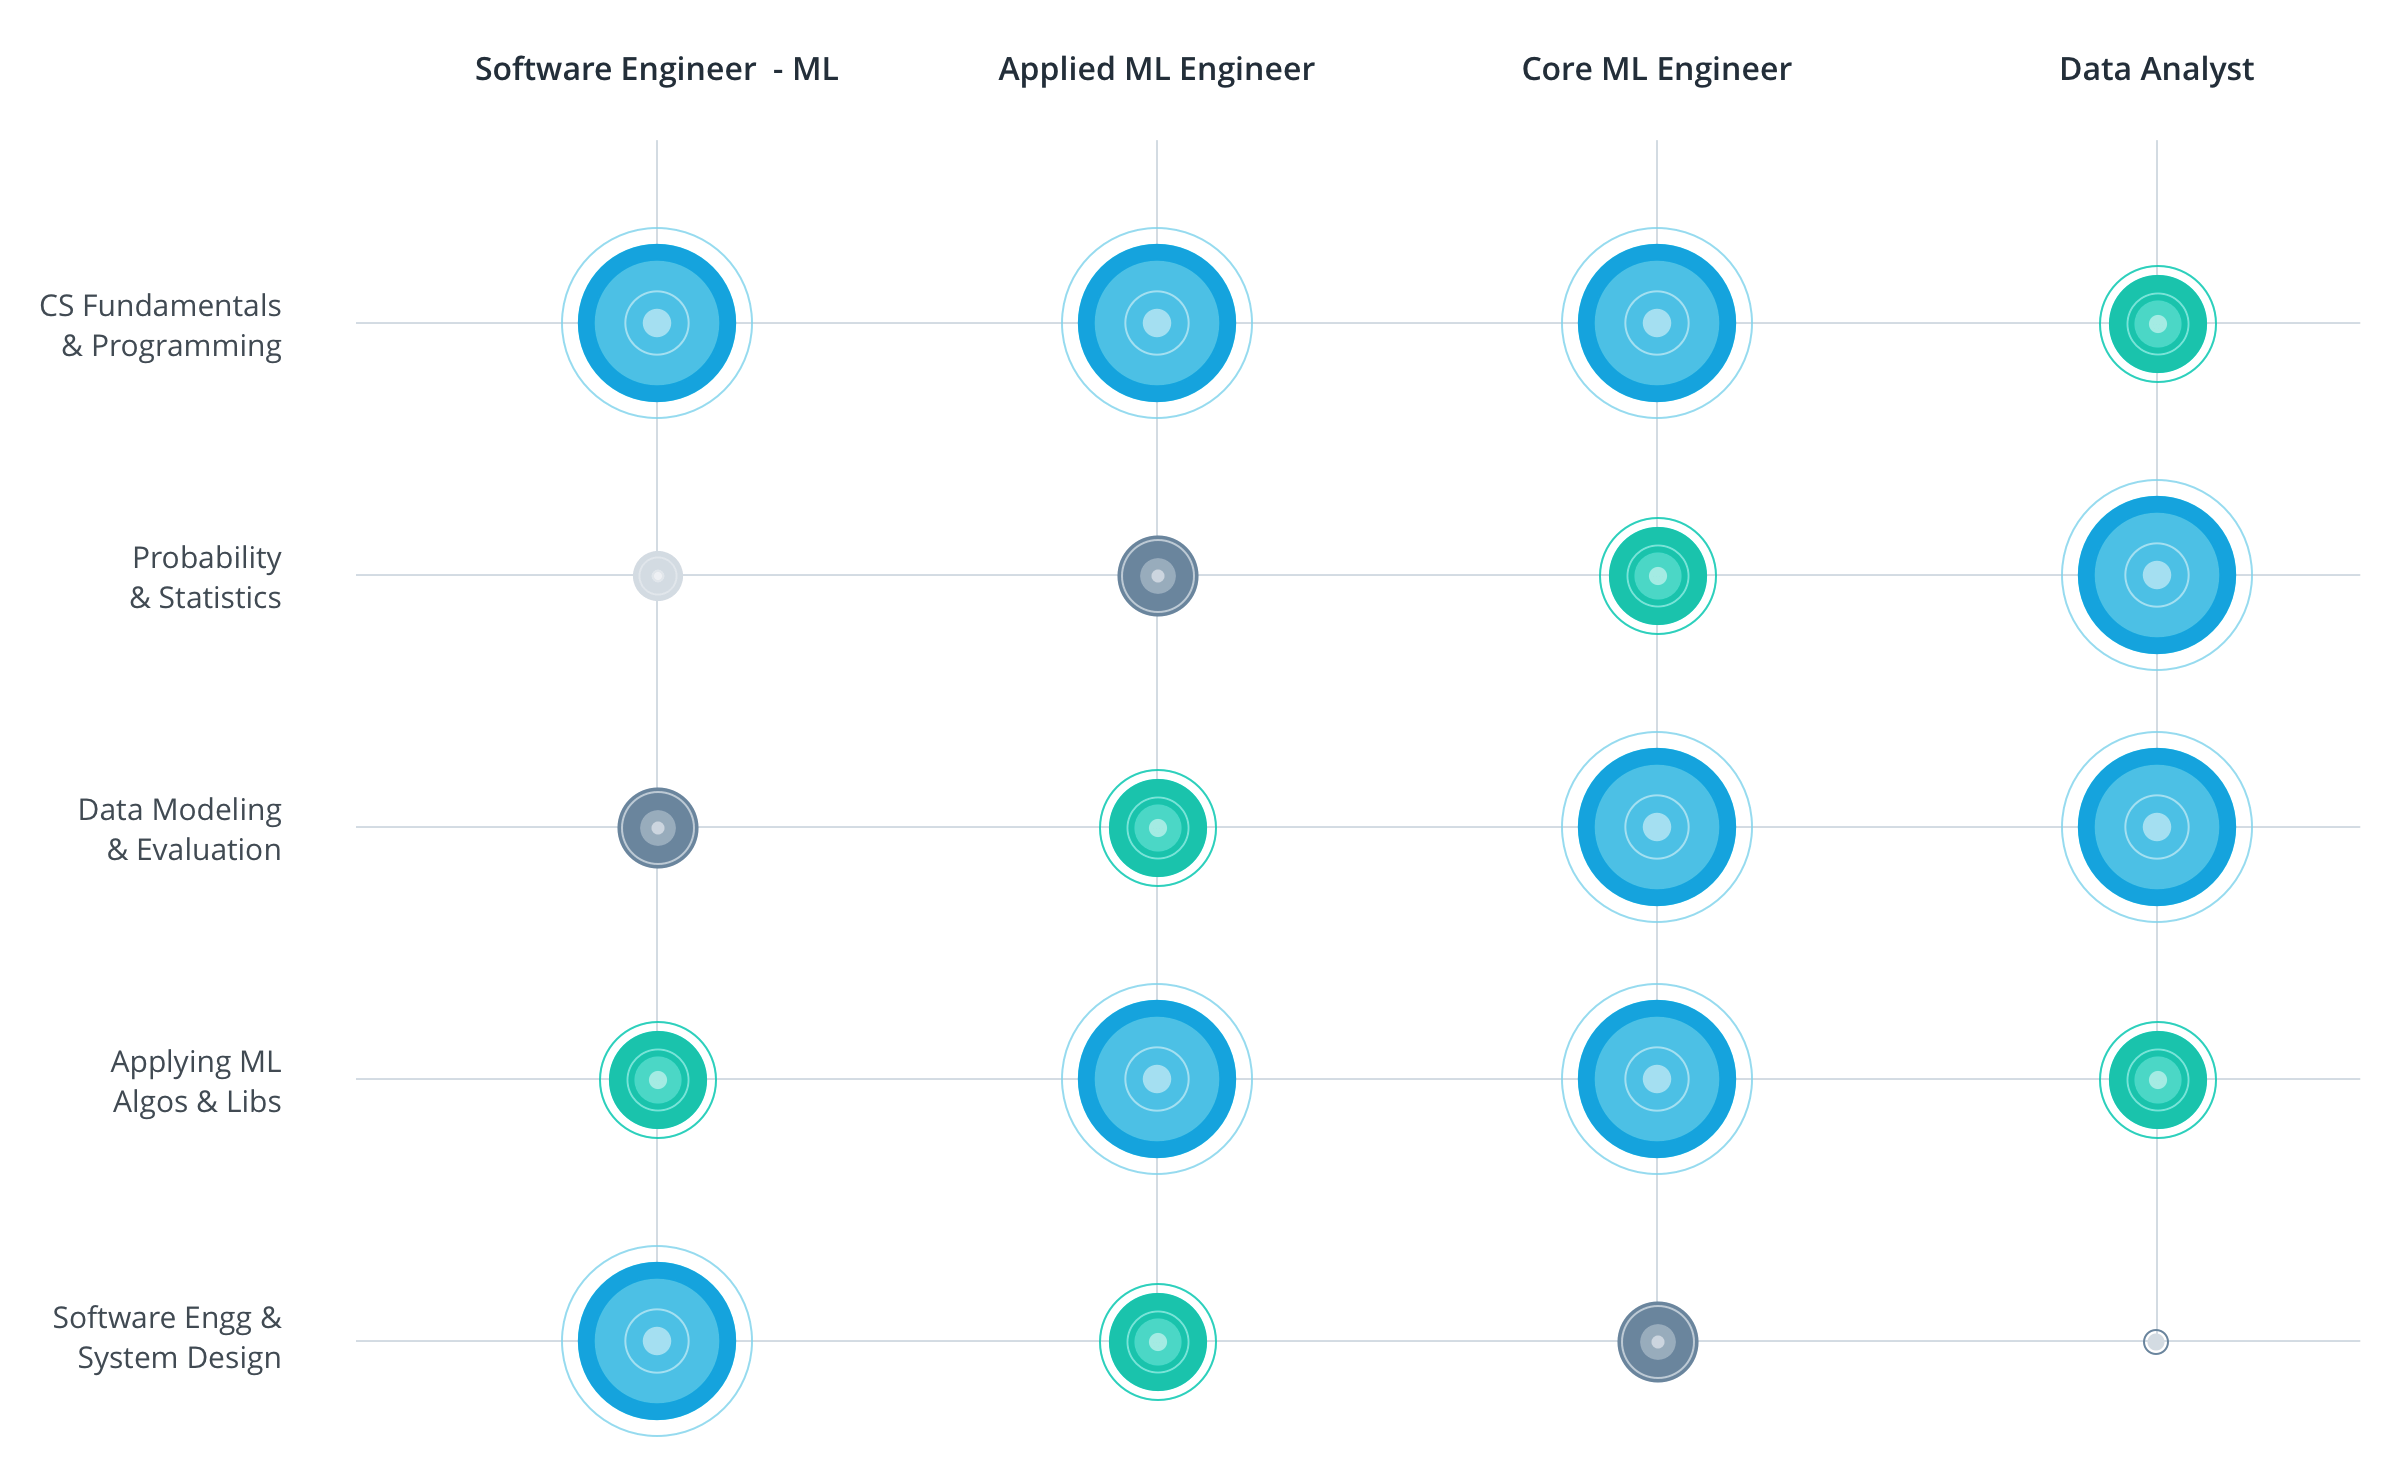
\includegraphics[width=0.8\textwidth]{imgs/cs-skills.png}
    \end{figure}
    \centering\tiny{Source: \url{https://blog.udacity.com/2016/04/5-skills-you-need-to-become-a-machine-learning-engineer.html}}
\end{frame}

\begin{frame}
    \textbf{Top seis trabajos con un grado en CS}
    \begin{itemize}
        \item[\small{1.}] Data Engineer (salario U.S. 137k\$)
        \item[\small{2.}] Machine Learning Engineer (salario U.S. 121k\$)
        \item[\small{3.}] Software Architect (salario U.S. 108k\$)
        \item[\small{4.}] Software Engineer (salario U.S. 105k\$)
        \item[\small{5.}] Mobile Application Developer (salario U.S. 90k\$)
        \item[\small{6.}] Full Stack Web Developer (salario U.S. 88k\$)
    \end{itemize}

    \tiny{Source: \url{https://blog.coursera.org/top-6-jobs-computer-science-degree/}}
\end{frame}


\section{Images}
\begin{frame}
\begin{itemize}[<+->]

    \item Machine learning, as part of IA,
    \item Second point
    \item Third point
\end{itemize}
	\frametitle{Slide 1}
	Content of slide 1
\end{frame}

\section{Tables}
\begin{frame}
	\frametitle{Slide 2}
\end{frame}

\section{References}
\begin{frame}
    \frametitle{How to use references}
    \shortciteNP{Ke2005} mentions that the Peter Pan is a creation of your imagination, however, it is also discussed that some people's imagination is not suitable to create such character \shortcite{Ke2005}.
\end{frame}

\section*{Bibliography}
\begin{frame}[allowframebreaks]
    \frametitle{References}
    \fontsize{5pt}{6.2}\selectfont
    \bibliographystyle{apacite}
    \renewcommand{\bibliographytypesize}{\small}
    \bibliography{presentation}
\end{frame}

\end{document}
\def\seminarname{Machine Learning Seminar}
\def\presentationtitle{Introducci\'on a Machine Learning}

\title{\large\seminarname:\\\large\presentationtitle}
\author{Author Name\\
    \small University
}

%Please make sure the tex is compiled twice to have all the images displayed correctly.

%Fill the date or leave it blank to not display it
\date{January 28th, 2019}

\begin{document}
\thispagestyle{empty}
%\begin{frame}[plain] %put [plain] at the end to get rid of the page number on this page
\begin{frame}
    \titlepage
\end{frame}

\begin{frame}
    \frametitle{Outline}
    \tableofcontents
\end{frame}

\AtBeginSection[]
{
    \begin{frame}<beamer>
    \frametitle{Outline}
    \tableofcontents[currentsection]
    \end{frame}
}

\section{Itemize}
\begin{frame}
\frametitle{Itemize}
\begin{itemize}[<+->]
    \item First point
    \item Second point
    \item Third point
\end{itemize}
\end{frame}

\section{Images}
\begin{frame}
	\frametitle{Slide 1}
	Content of slide 1
\end{frame}

\section{Tables}
\begin{frame}
	\frametitle{Slide 2}
\end{frame}

\section{References}
\begin{frame}
    \frametitle{How to use references}
    \shortciteNP{Ke2005} mentions that the Peter Pan is a creation of your imagination, however, it is also discussed that some people's imagination is not suitable to create such character \shortcite{Ke2005}.
\end{frame}

\section*{Bibliography}
\begin{frame}[allowframebreaks]
    \frametitle{References}
    \fontsize{5pt}{6.2}\selectfont
    \bibliographystyle{apacite}
    \renewcommand{\bibliographytypesize}{\small}
    \bibliography{presentation}
\end{frame}

\end{document}
